\documentclass[]{article}

% Package
\usepackage{amsmath}
\usepackage{breqn}
\usepackage[english]{babel}
\usepackage{graphicx}

%opening
\title{SC4045: Deformable Mirror}
\author{Yudha Prawira Pane - 4321499}

\begin{document}

\maketitle

\begin{abstract}

\end{abstract}

\section{Constructing H Matrix}
The $ H $ matrix is constructed by calculating the influence function $ S(x,y) $ for each of its element. The function is formulated as follows:
\begin{dmath}
S(x,y) = \left\lbrace \frac{w_1}{2\pi \sigma^2_1}exp\left[\frac{-((x-posAct_x[i])^2 + (x-posAct_y[i])^2)}{2\sigma^2_1} \right]  +  \frac{w_2}{2\pi \sigma^2_2}exp\left[\frac{-((x-posAct_x[i])^2 + (x-posAct_y[i])^2)}{2\sigma^2_2} \right] \right\rbrace 0.470 \mu m
\end{dmath}

$ posAct_x[i] $ and $ PosAct_y[j] $ is $ x $ and $ y $ coordinate $ i $-th actuator. This function basically looks like a 2D gaussian distribution whose mean is the position of the actuators (assuming position as a point) and variance are $ sigma_1 $ and $ sigma_2 $. To get an insight about the mirror's shape, figure  is what the mirror looks like when one of the actuators is "poked".

\begin{figure}[h!]
\centering
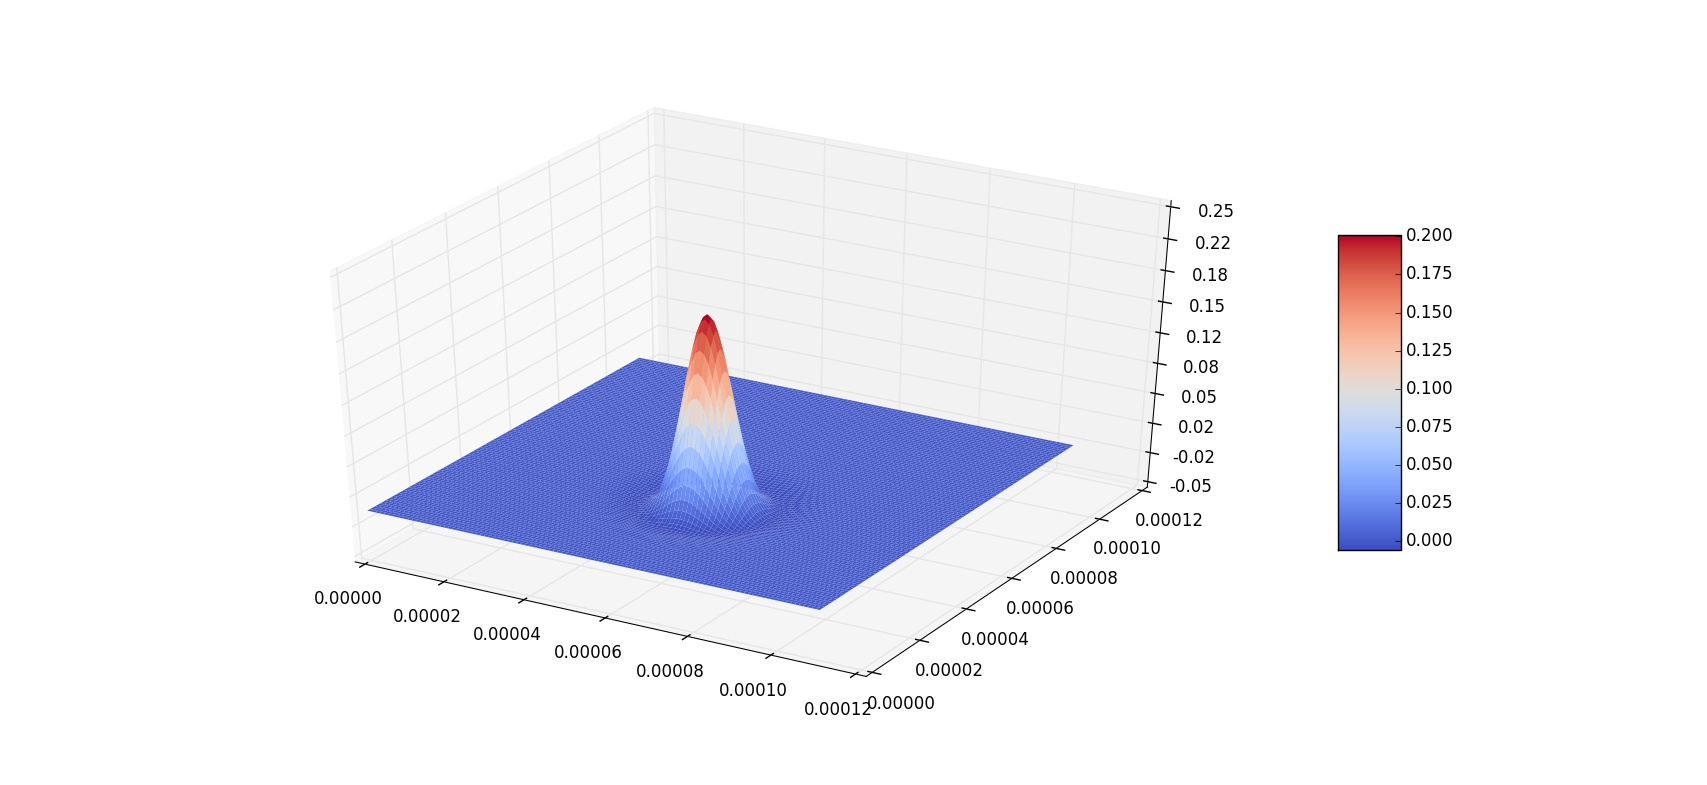
\includegraphics[width=0.7\linewidth]{fig1}
\caption{Mirror shape when one actuator is "poked'}
\label{fig1}
\end{figure}

\section{Estimating the Best Actuators Input}
The deformable mirror's phase $ \phi_{DM} $ and actuator inputs u is related according the following equation:
\begin{equation}
\phi_{DM} = Hu
\label{eqdm}
\end{equation}
Where $ \phi_{DM} \in \mathcal{R}^m $, $ u = \in \mathcal{R}^n $, $ H \in \mathcal{R}^{mxn} $ and $ m>n $.

Now, given estimated wavefront $ \phi $ from wavefront reconstruction block, calculate u that best approximates this wavefront using linear least square principle.

\begin{equation}
u = (H^TH)^{-1}H^T\hat{\phi}
\end{equation}

Therefore, $ \phi_{DM} $ is then obtained by \ref{eqdm}.

\section{Hard-coded Example}

To demonstrate that above method indeed works, the following scenario is hard-programmed. First, the number of wavefront and its spacing is determined as 144 and 8.46$ \mu $ m respectively. Second, the wavefront is generated based on random function and fed to the DM block. The number of wavefront (144) is larger than the number of actuators (100). The incoming wavefront and actuators are positioned as shown in figure \ref{fig2} by assuming that the mirror is a rectangular shaped.

\begin{figure}[h!]
\centering
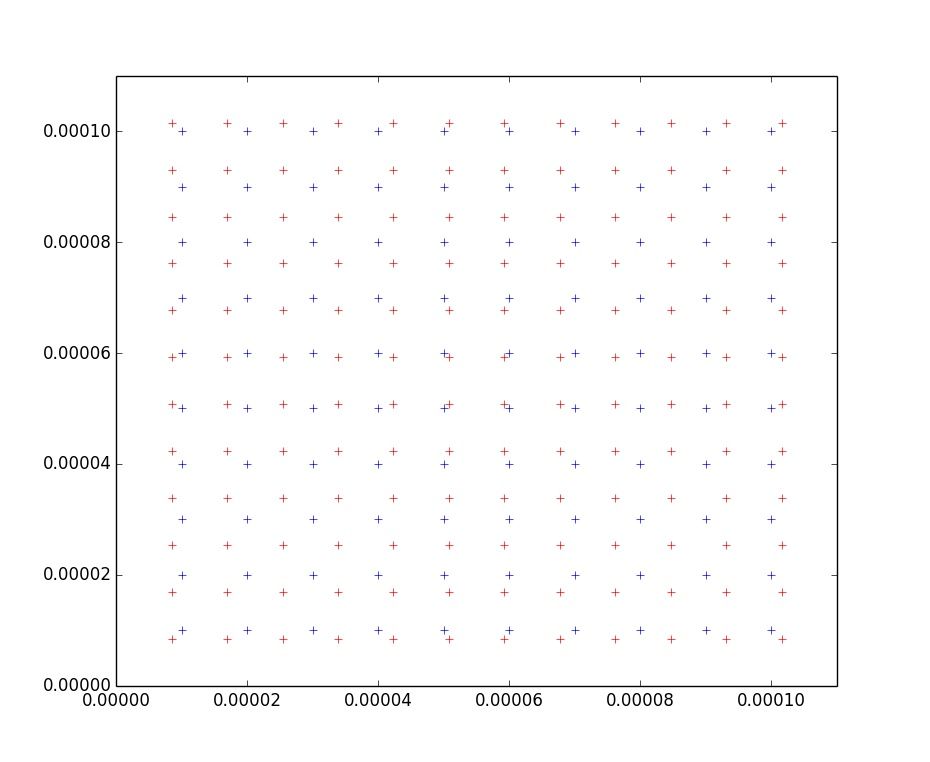
\includegraphics[width=0.7\linewidth]{fig2}
\caption{Position of actuators (blue) and wavefront (red)}.
\label{fig2}
\end{figure}

The "best" actuators input is then estimated and the $ \phi_{DM} $ is calculated. The surface of the deformable mirror which approximates the wavefront is shown in figure below.

\begin{figure}[h!]
\centering
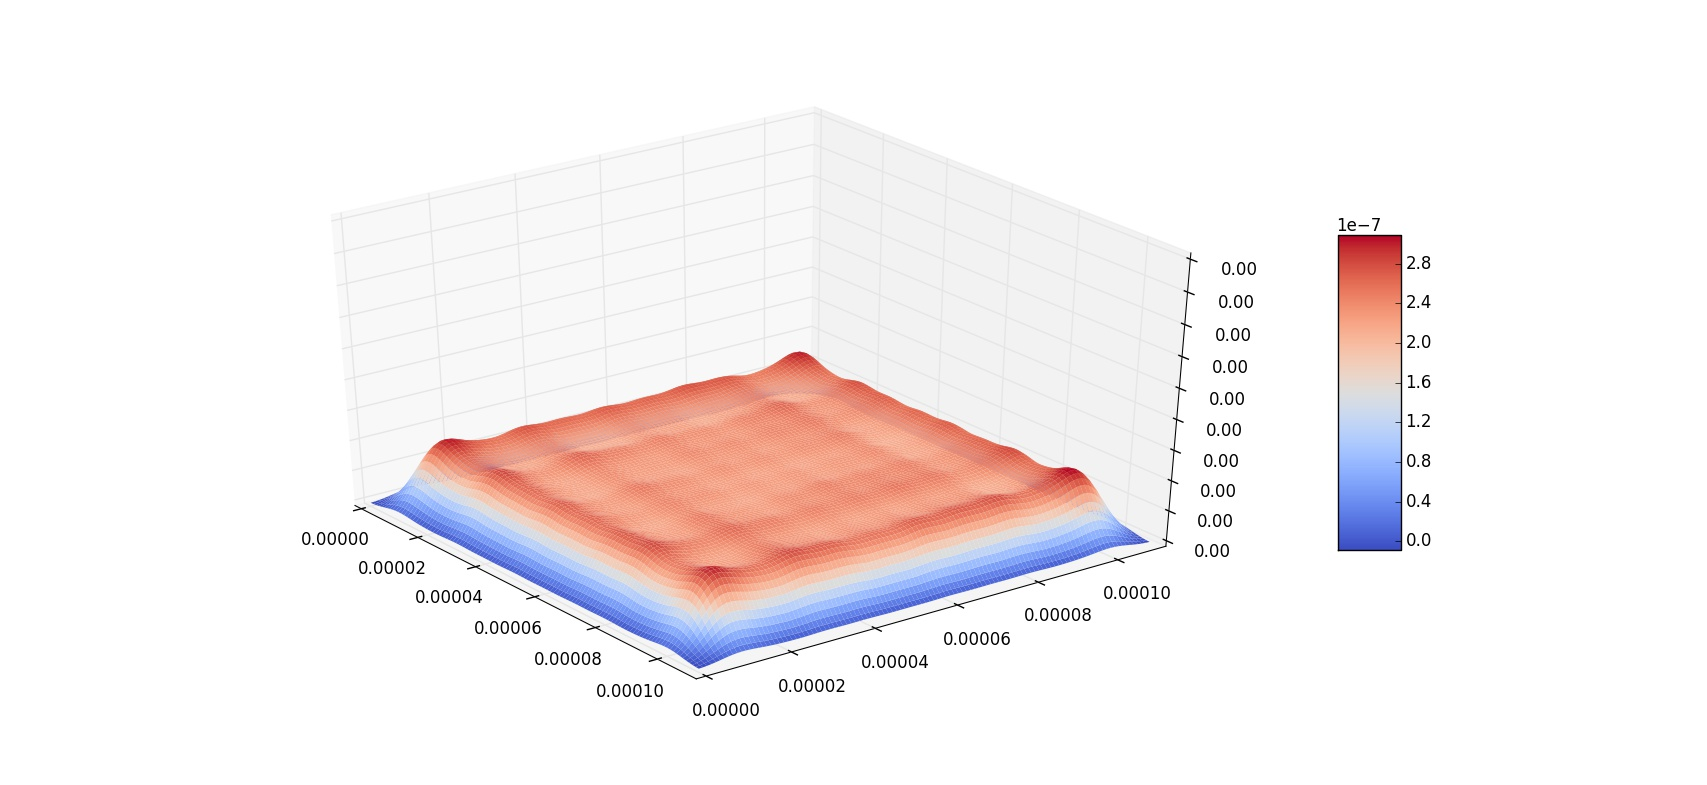
\includegraphics[width=1\linewidth]{fig3}
\caption{Deformable mirror shape as an estimate of reconstructed wavefront}.
\label{fig3}
\end{figure}

\end{document}
